\newcommand{\psd}[1]{{\small\sffamily{\color{blue!60}#1}}}

To showcase the usage of linear elasticity, we shall discuss here an
example of a 2D bar which bends under its own load (body weight). The
bar 5 m in length and 1 m in width, and is supposed to be made up of a
material with density \(\rho=8\times 10^3\), Youngs modulus
\(E=200\times 10^9\), and Poissons ratio \(\nu=0.3\).
\Cref{2dbar-le-full} shows this bar considered in this tutorial.

\begin{figure}[h!]
\centering
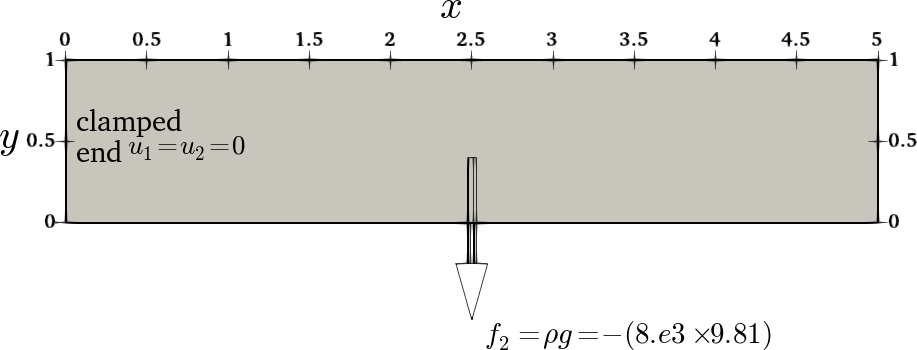
\includegraphics[width=0.5\textwidth]{./Images/le-2d-bar.png}
\caption{The 2D clamped bar problem. \label{2dbar-le-full}}
\end{figure}

\subsection{Step 1: Preprocessing}

First step in a PSD simulation is PSD preprocessing, at this step you
tell PSD what kind of physics, boundary conditions, approximations,
mesh, etc are you expecting to solve. PSD is a TUI (terminal user
interface) based application, so the user needs to use the terminal
(command-line) to communicate to PSD.

In the terminal \psd{cd} to the folder
\psd{/home/PSD-tutorials/linear-elasticity}
\footnote{Note that one can perform these simulation in any folder provided that PSD has been properly installed. We use \psd{/home/PSD-tutorials/linear-elasticity} for simplicity, once the user is proficient a simulation can be launch elsewhere.}.
Launch \psd{PSD\_PreProcess} with some falsgs from the terminal, to do
so run the following command.

\begin{lstlisting}[style=BashInputStyle]
PSD_PreProcess -problem linear_elasticity -dimension 2 -bodyforceconditions 1 \
-dirichletconditions 1 -postprocess u
\end{lstlisting}

\textbf{What do the arguments mean ?}

\begin{itemize}
\item \psd{-problem linear\_elasticity} means that we are solving a linear elasticity problem;
\item \psd{-dimension 2} means it is a 2D simulation;
\item \psd{-bodyforceconditions 1} with applied body force (body weight) acting on the domain;
\item \psd{-dirichletconditions 1} says we have one Dirichlet border (clamped end);
\item \psd{-postprocess u} means we would like to have ParaView post processing files.
\end{itemize}

After the \psd{PSD\_PreProcess} runs successfully you should see many
\psd{.edp} files in your current folder. You will now have to follow an
edit cycle, where you will provide PSD with some other additional
information about your simulation that you wish to perform - in this
case 2D linear elasticity bending under its own body weight.

At this stage the input properties of Youngs modulus and Poissons ratio
(\(E,\nu\)) can be mentioned in \psd{ControlParameters.edp}, use
\psd{E = 200.e9}, and \psd{nu = 0.3;}. The volumetric body force
condition is mentioned in the same file via variable
\psd{Fbc0Fy -78480.0}, i.e (\(\rho*g=8.e3*(-9.81)=-78480.0\)). One can
also provide the mesh to be used in \psd{ControlParameters.edp}, via
\psd{ThName = "../Meshes/2D/bar.msh"}\footnote{Note that mesh can also be provided in the next step i.e, Step 2: solving.}.
In addition variable \psd{Fbc0On 1} has to be provided in order to
indicate the volume (region) for which the body force is acting, here
\psd{1} is the integer volume tag of the mesh. Dirichlet boundary
conditions are also provided in \psd{ControlParameters.edp}. To provide
the clamped boundary condition the variables \psd{Dbc0On 2},
\psd{Dbc0Ux 0.}, and \psd{Dbc0Uy 0.} are used, which means for Dirichlet
border \psd{2} (\psd{Dbc0On 2}) where \psd{2} is the clamped border
label of the mesh Dirichlet constrain is applied and \psd{Dbc0Ux 0.},
\psd{Dbc0Uy 0} i.e., the clamped end condition (\(u_x=u_y=0\)).

Please note that for this simple problem, the bar mesh (\psd{bar.msh})
has been provided in \psd{../Meshes/2D/"} folder, this mesh is a
triangular mesh produced with Gmsh. Moreover detailing meshing procedure
is not the propose of PSD tutorials. A user has the choice of performing
their own meshing step and providing them to PSD in
\psd{.msh}\footnote{Please use version 2} or \psd{.mesh} format, we
recommend using Salome or Gmsh meshers for creating your own geometry
and meshing them.

\subsection{Step 2: Solving}

As PSD is a parallel solver, let us use 4 cores to solve the 2D bar
case. To do so enter the following command:

\begin{lstlisting}[style=BashInputStyle]
PSD_Solve -np 4 Main.edp -mesh ./../Meshes/2D/bar.msh -v 0
\end{lstlisting}

This will launch the PSD simulation.

Here \psd{-np 4} (number of processes) denote the argument used to enter
the number of parallel processes (MPI processes) used by PSD while
solving. \psd{-mesh ./../Meshes/2D/bar.msh} is used to provide the mesh
file to the
solver\footnote{ \psd{-mesh} argument is not needed if the user has indicated the right mesh in \psd{ControlParameters.edp} file}.
\psd{-v 0} denotes the verbosity level on screen. \psd{PSD\_Solve} is a
wrapper around \psd{FreeFem++-mpi}. Note that if your problem is large
use more cores. PSD has been tested upto 24,000 parallel processes (on
the French Joliot-Curie supercomputer) and problem sizes with billions
of unknowns, surely you will not need that many for the 2D bar problem.

\subsection{Step 3: Postprocessing}

PSD allows postprocessing of results in ParaView. After the step 2
mentioned above finishes. Launch ParaView and have a look at the
\psd{.pvd} file in the \psd{VTUs...} folder. Using ParaView for
postprocessing the results that are provided in the \psd{VTUs...}
folder, results such as those shown in \cref{bar-le-full-1} can be
extracted.

\begin{figure}[h!]
\centering
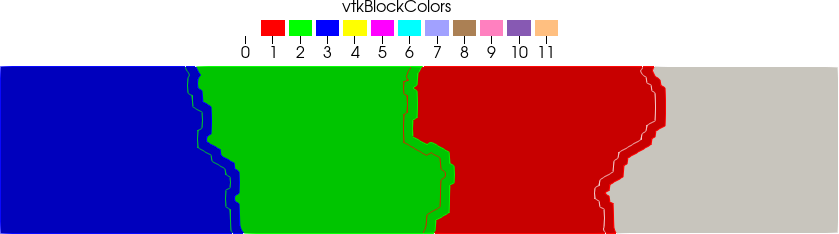
\includegraphics[align=t,width=0.4\textwidth]{./Images/le-2d-bar-partioned.png}\hfill
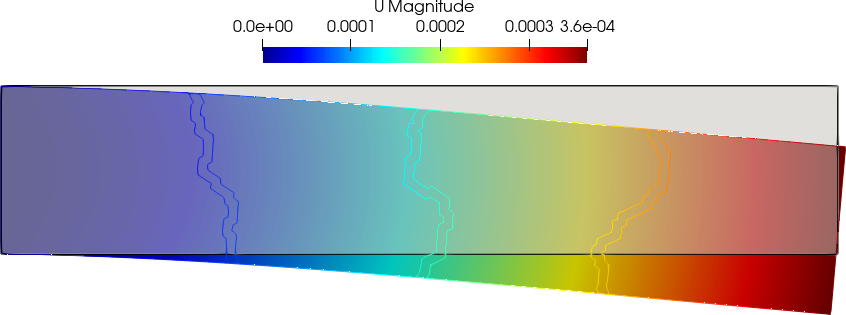
\includegraphics[align=t,width=0.4\textwidth]{./Images/le-2d-bar-results.png}
\caption{The 2D clamped bar problem: partitioned mesh and displacement field visualization in ParaView. \label{bar-le-full-1}}
\end{figure}

You are all done with your 2D linear-elasticty simulation.

\subsection{2D bar is ok, but what about 3D ?}

In PSD a 3D simulation follows the same logic as a 2D one, in the
preprocessing step. Imagine the same problem as above, however now the
geometry is 3D with length 5 m and cross sectional area 1 m \(\times\) 1
m. Indeed all what changes for this simulation is the geometry
(consequently the mesh) and the dimension of the problem, these two
changes will be handled by (\psd{-dimension} and \psd{-mesh}) arguments.

The preprocessing step now becomes:

\begin{lstlisting}[style=BashInputStyle]
PSD_PreProcess -problem linear_elasticity -dimension 3 -bodyforceconditions 1 \
-dirichletconditions 1 -postprocess u
\end{lstlisting}

compared to the 2D problem, note that all what has changed
\psd{-dimension 3} instead of \psd{-dimension 2}.

Solving step remains exactly the same with except \psd{-mesh} flag now
pointing towards the 3D mesh of the bar.

\begin{lstlisting}[style=BashInputStyle]
PSD_Solve -np 4 Main.edp -mesh ./../Meshes/3D/bar.msh -v 0
\end{lstlisting}

\begin{figure}[h!]
\centering
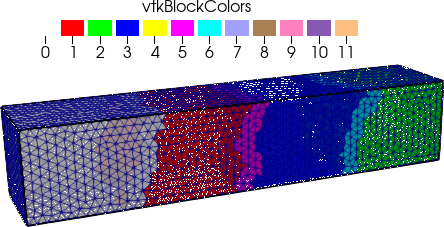
\includegraphics[width=0.4\textwidth]{./Images/le-3d-bar-clamped-ends.png}\\
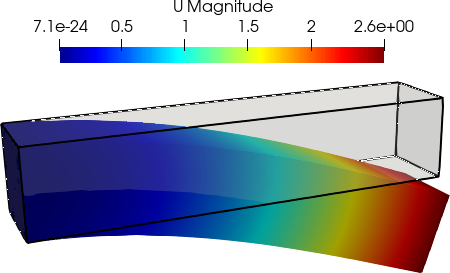
\includegraphics[width=0.4\textwidth]{./Images/le-3d-bar-clamped-pulled-partioned.png}
\caption{The 3D clamped bar problem: partitioned mesh and displacement field visualization in ParaView. \label{3dbar-le-full}}
\end{figure}

Finally, using ParaView for postprocessing the results that are provided
in the \psd{VTUs...} folder, results such as those shown in
\cref{3dbar-le-full} can be extracted.
